\documentclass{article}

\usepackage{color}
\usepackage{graphicx}
\usepackage{amsmath}
\usepackage{geometry}
\usepackage{setspace}
\usepackage{indentfirst}
\usepackage{listings}
\usepackage{xcolor}
\lstset{
    columns=fixed,       
    numbers=left,                                       
    frame=none,                                          
    backgroundcolor=\color[RGB]{245,245,244},            
    keywordstyle=\color[RGB]{40,40,255},                 
    numberstyle=\footnotesize\color{darkgray},           
    commentstyle=\it\color[RGB]{0,96,96},                
    stringstyle=\rmfamily\slshape\color[RGB]{128,0,0},   
    showstringspaces=false,                              
    language=c++,                                        
}
\geometry{left=2cm,right=2cm,top=2cm,bottom=2cm}
\begin{document}
\begin{spacing}{2.0}
\vspace*{0.25cm}

\hrulefill

\thispagestyle{empty}

\begin{center}
\begin{large}
\sc{UM--SJTU Joint Institute \vspace{0.3em} \\ Data Structures and Algorithms \\(VE281)}
\end{large}

\hrulefill

\vspace*{5cm}
\begin{Large}
\sc{{Homework 2}}
\end{Large}

\vspace{2em}

\end{center}


\vfill

\begin{table}[h!]
\flushleft
\begin{tabular}{lll}
Name: Ji Xingyou \hspace*{2em}&
ID: 515370910197\hspace*{2em}
\\

Date: 10 October 2017

\end{tabular}
\end{table}

\hfill

\newpage
\tableofcontents
\newpage
\section{Theoretical Data}
\indent As is discussed in the class, we can get the following table summarizing the time complexity for each algorithms.

\begin{table}[!hbp]
\centering
\begin{tabular}{ccccc}
&Worst case complexity&Average case complexity&In place&Stable\\
\hline
\hline
Quick sort in place&$O(N^2)$&$O(NlogN)$&Yes&No\\
\hline
Rselect&$\Theta(n^2)$&$O(N)$&Yes&Yes\\
\hline
Dselect&&$O(N)$&No&Yes\\
\hline
\end{tabular}
\caption{Time complexity of comparison sorting}
\end{table}

In this report, we will first implement all these three algorithms, and then test the run time for each of them to see whether the above table makes sense.

The implementation of the algorithms is attached in the appendix.
\section{Result Analysis}
\indent After finishing implementing the above three algorithms, I wrote another program to test the run time of each algorithm. In this program, I set two clocks, noting the starting and finishing instance. To avoid uncertainty in the data, I wrote a while loop to run the program 10 times so that I could get the average value. There is one thing which requires extra carefulness. That is, we must ensure that every time inside the while loop, all the six sorting should meet the identical array. Otherwise, you will see that insertion sort will have a leading performance no matter how large the size is.

The array size I chose is 10, 100, 1000, 5000, 10000, 50000, 100000 and 1000000.

The run time data for each algorithms is listed in table 2.
\begin{table}[!h]
\centering
\begin{tabular}{c|cccccc}
Array size&Quick sort in place&Rselect&Dselect\\
\hline
\hline
10&1&1&2\\
\hline
100&17&4&16\\
\hline
1000&154&24&152\\
\hline
5000&923&158&749\\
\hline
10000&2053&355&1498\\
\hline
50000&9853&1243&6046\\
\hline
100000&19602&2004&11323\\
\hline
1000000&206184&25104&100056\\
\hline
\end{tabular}
\caption{Run time of linear time selection}
\end{table}

The run time comparison is shown in figure 1. 
\begin{figure}[h!]
\begin{center}
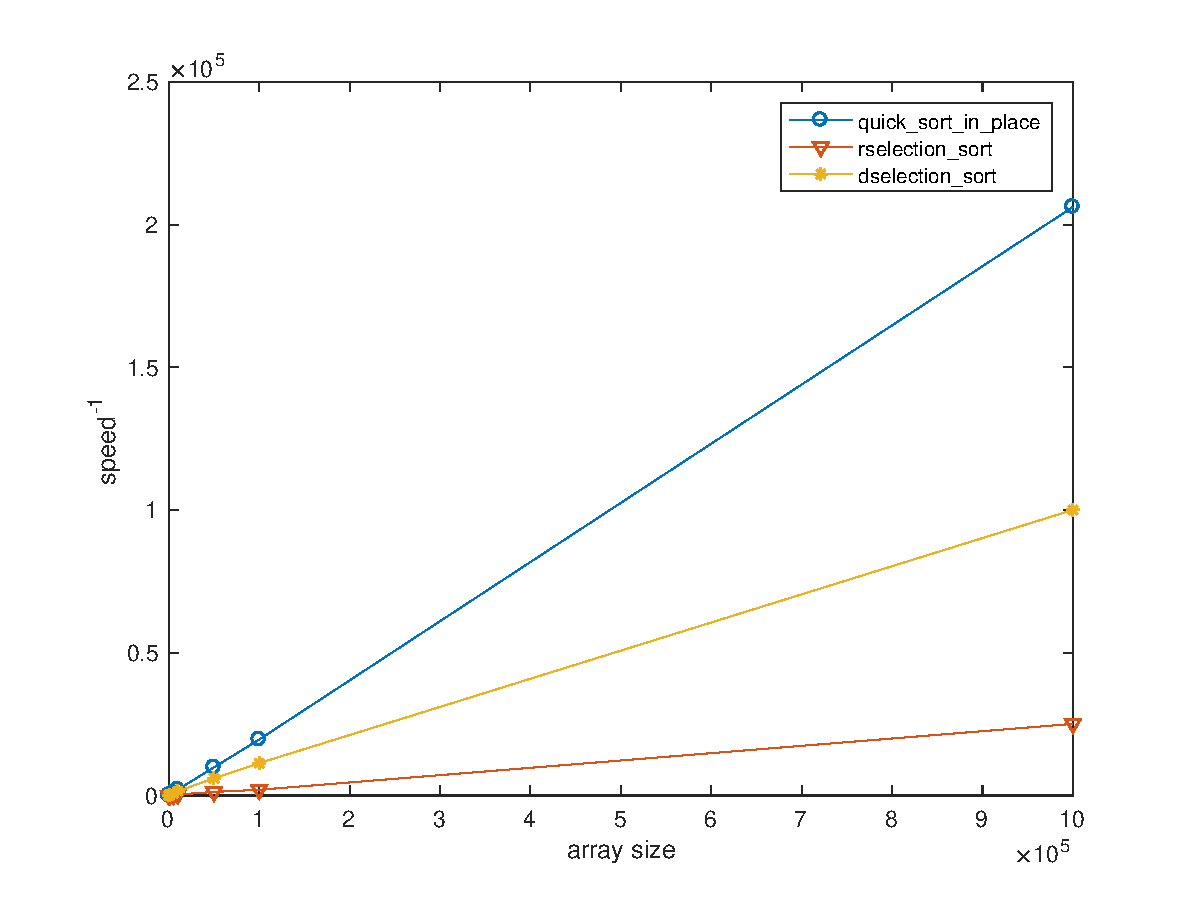
\includegraphics[scale=1]{comparision.eps}
\caption{Run time comparison}
\end{center}
\end{figure}

Combining the table and figure above, we can conclude the following points.
\begin{enumerate}
\item For each linear time selection algorithm, the run time increases as the size of the array increases.\\
\item For any given array size, Rselect always has a leading performance, while Dselect ranks second and quick sort third.
\end{enumerate}

From the conclusion listed above, we can see that it fits the time complexity shown in table 1, which means the algorithms make sense.

This inspires me that in future learning, when dealing with selection, I should use Rselect as often as possible since it has the best performance.
\section{Appendix}
\subsection{Linear time selection algorithms}
\begin{lstlisting}[language=c++]
//
//  main.cpp
//  project2
//
//  Created by 季星佑 on 2017/9/27.
//  Copyright © 2017年 季星佑. All rights reserved.
//

#include <iostream>
#include <fstream>
#include <sstream>
#include <string>
#include <cstdlib>
#include <climits>
#include <ctime>
#include <cassert>

using namespace std;

int Rselect(int *arr,int n,int i);

int Dselect(int *arr,int n,int i);

int partition(int *arr,int left,int right,int size,int pivotat);

void selection_sort(int *arr,int n);
//////////////////////////////
//////////////////////////////
int main(int argc, const char * argv[])
{
    int choice;
    cin>>choice;
    int n;
    cin>>n;
    if(n==0)
    {
        return 0;
    }
    int i;
    cin>>i;
    if(i>=n||i<0)
    {
        return 0;
    }
    int a[n];
    for(int t=0;t<n;++t)
    {
        cin>>a[t];
    }
    int *arr=a;
    int result=0;
    switch(choice)
    {
        case 0:
            result=Rselect(arr,n,i);
            break;
        case 1:
            result=Dselect(arr,n,i);
        default:
            break;
    }
    cout<<"The order-"<<i<<" item is "<<result<<endl;
//    srand(time(0));
//    int times=100;
//    while(times--)
//    {
//        int size=100;
//        int index=rand()%size;
//        int *arr=new int [size];
//        int brr[size];
//        for(int i=0;i<size;++i)
//        {
//            arr[i]=rand()%size;
//        }
//        for(int i=0;i<size;++i)
//        {
//            brr[i]=arr[i];
//        }
//        sort(arr,arr+size);
//        int p=arr[index];
//        int q=Rselect(brr,size,index);
//        cout<<p-q<<endl;
//        delete [] arr;
//    }
    return 0;
}
//////////////////////////////
//////////////////////////////
int Rselect(int *arr,int n,int i)
{
    if(n==1)
    {
        return *arr;
    }
    int pivotat=rand()%n;
    pivotat=partition(arr,0,n-1,n,pivotat);
    if(pivotat==i)
    {
        return arr[pivotat];
    }
    else if(pivotat>i)
    {
        return Rselect(arr,pivotat,i);
    }
    else
    {
        return Rselect(arr+pivotat+1,n-pivotat-1,i-pivotat-1);
    }
}
//////////////////////////////
//////////////////////////////
int Dselect(int *arr,int n,int i)
{
    if(n<=1)
    {
        return *arr;
    }
    int group_num=n/5;
    int last=n%5;
    if(last==0)
    {
        last=5;
    }
    else
    {
        group_num++;
    }
    int *C=new int[group_num];
    int *temp=new int[5];
    int size=0;
    for(int p=0;p<group_num;++p)
    {
        if(p==group_num-1)
        {
            size=last;
        }
        else
        {
            size=5;
        }
        for(int q=0;q<size;++q)
        {
            temp[q]=arr[q+5*p];
        }
        selection_sort(temp,size);
        C[p]=temp[size/2];
    }
    int pivot=Dselect(C,n/5,n/10);
    delete [] C;
    delete [] temp;
    int pivotat=0;
    for(int p=0;p<n;++p)
    {
        if(arr[p]==pivot)
        {
            pivotat=p;
        }
    }
    pivotat=partition(arr,0,n-1,n,pivotat);
    if(pivotat==i)
    {
        return arr[pivotat];
    }
    else if(pivotat>i)
    {
        return Dselect(arr,pivotat,i);
    }
    else
    {
        return Dselect(arr+pivotat+1,n-pivotat-1,i-pivotat-1);
    }
}
//////////////////////////////
//////////////////////////////
int partition(int *arr,int left,int right,int size,int pivotat)
{
    swap(arr[0],arr[pivotat]);
    int i=1;
    int j=size-1;
    while(true)
    {
        while(i<size-1&&arr[i]<arr[0])
        {
            ++i;
        }
        while(j>0&&arr[j]>=arr[0])
        {
            --j;
        }
        if(i<j)
        {
            swap(arr[i],arr[j]);
        }
        else
        {
            break;
        }
    }
    swap(arr[0],arr[j]);
    return j;
}
//////////////////////////////
//////////////////////////////
void selection_sort(int *arr,int n)
{
    for(int i=0;i<n-1;++i)
    {
        int index=i;
        for(int j=i+1;j<n;++j)
        {
            if(arr[j]<arr[index])
            {
                index=j;
            }
        }
        if(index!=i)
        {
            int tmp=arr[index];
            arr[index]=arr[i];
            arr[i]=tmp;
        }
    }
}


\end{lstlisting}
\subsection{Run-time calculation}
\begin{lstlisting}[language=c++]
//
//  main.cpp
//  run_time_study
//
//  Created by 季星佑 on 2017/10/9.
//  Copyright © 2017年 季星佑. All rights reserved.
//

#include <iostream>
#include <fstream>
#include <sstream>
#include <string>
#include <cstdlib>
#include <climits>
#include <ctime>
#include <cassert>

using namespace std;

int Rselect(int *arr,int n,int i);

int Dselect(int *arr,int n,int i);

int partition(int *arr,int left,int right,int size,int pivotat);

void selection_sort(int *arr,int n);

void quick_sort_in_place(int *arr,int left,int right,int size);
//////////////////////////////
//////////////////////////////
int main(int argc, const char * argv[])
{
    int lines=1000000;
    srand(time(0));
    int index=rand()%lines;
    long temp0=0;
    long temp1=0;
    long temp2=0;
    clock_t start,finish;
    int arr[lines];
    for(int i=0;i<lines;++i)
    {
        arr[i]=rand();
    }
    int brr[lines];
    for(int j=0;j<lines;++j)
    {
        brr[j]=arr[j];
    }
    int k=0;
    while(k<10)
    {
        //////////////////////////////
        start=clock();
        for(int a=0;a<lines;++a)
        {
            arr[a]=brr[a];
        }
        quick_sort_in_place(arr,0,lines-1,lines);
        int p=arr[index];
        finish=clock();
        long t0=finish-start;
        temp0+=t0;
        //////////////////////////////
        start=clock();
        for(int a=0;a<lines;++a)
        {
            arr[a]=brr[a];
        }
        Rselect(arr,lines,index);
        finish=clock();
        long t1=finish-start;
        temp1+=t1;
        //////////////////////////////
        start=clock();
        for(int a=0;a<lines;++a)
        {
            arr[a]=brr[a];
        }
        Dselect(arr,lines,index);
        finish=clock();
        long t2=finish-start;
        temp2+=t2;
        //////////////////////////////
        k++;
    }
    long time0=temp0/10;
    long time1=temp1/10;
    long time2=temp2/10;
    cout<<time0<<endl;
    cout<<time1<<endl;
    cout<<time2<<endl;
    return 0;
}
//////////////////////////////
//////////////////////////////
int Rselect(int *arr,int n,int i)
{
    if(n==1)
    {
        return *arr;
    }
    int pivotat=rand()%n;
    pivotat=partition(arr,0,n-1,n,pivotat);
    if(pivotat==i)
    {
        return arr[pivotat];
    }
    else if(pivotat>i)
    {
        return Rselect(arr,pivotat,i);
    }
    else
    {
        return Rselect(arr+pivotat+1,n-pivotat-1,i-pivotat-1);
    }
}
//////////////////////////////
//////////////////////////////
int Dselect(int *arr,int n,int i)
{
    if(n<=1)
    {
        return *arr;
    }
    int group_num=n/5;
    int last=n%5;
    if(last==0)
    {
        last=5;
    }
    else
    {
        group_num++;
    }
    int *C=new int[group_num];
    int *temp=new int[5];
    int size=0;
    for(int p=0;p<group_num;++p)
    {
        if(p==group_num-1)
        {
            size=last;
        }
        else
        {
            size=5;
        }
        for(int q=0;q<size;++q)
        {
            temp[q]=arr[q+5*p];
        }
        selection_sort(temp,size);
        C[p]=temp[size/2];
    }
    int pivot=Dselect(C,n/5,n/10);
    delete [] C;
    delete [] temp;
    int pivotat=0;
    for(int p=0;p<n;++p)
    {
        if(arr[p]==pivot)
        {
            pivotat=p;
        }
    }
    pivotat=partition(arr,0,n-1,n,pivotat);
    if(pivotat==i)
    {
        return arr[pivotat];
    }
    else if(pivotat>i)
    {
        return Dselect(arr,pivotat,i);
    }
    else
    {
        return Dselect(arr+pivotat+1,n-pivotat-1,i-pivotat-1);
    }
}
//////////////////////////////
//////////////////////////////
int partition(int *arr,int left,int right,int size,int pivotat)
{
    swap(arr[0],arr[pivotat]);
    int i=1;
    int j=size-1;
    while(true)
    {
        while(i<size-1&&arr[i]<arr[0])
        {
            ++i;
        }
        while(j>0&&arr[j]>=arr[0])
        {
            --j;
        }
        if(i<j)
        {
            swap(arr[i],arr[j]);
        }
        else
        {
            break;
        }
    }
    swap(arr[0],arr[j]);
    return j;
}
//////////////////////////////
//////////////////////////////
void selection_sort(int *arr,int n)
{
    for(int i=0;i<n-1;++i)
    {
        int index=i;
        for(int j=i+1;j<n;++j)
        {
            if(arr[j]<arr[index])
            {
                index=j;
            }
        }
        if(index!=i)
        {
            int tmp=arr[index];
            arr[index]=arr[i];
            arr[i]=tmp;
        }
    }
}

void quick_sort_in_place(int *arr,int left,int right,int size)
{
    if(size==0)
    {
        return;
    }
    int pivotat=rand()%size;
    if(left>=right)
    {
        return;
    }
    pivotat=partition(arr,left,right,size,pivotat);
    quick_sort_in_place(arr,left,pivotat-1,pivotat-left);
    quick_sort_in_place(arr+pivotat+1,0,right-pivotat-1,right-pivotat);
}
\end{lstlisting}
\subsection{Visualization}
\begin{lstlisting}[language=Matlab]
clear all;clc;
t0=[1 17 154 923 2053 9853 19602 206184];
t1=[1 4 24 158 355 1243 2004 25104];
t2=[2 16 152 749 1498 6046 11323 100056];
size=[10 100 1000 5000 10000 50000 100000 1000000];
plot(size,t0,'o-',size,t1,'v-',size,t2,'*-');
xlabel('array size');
ylabel('speed^{-1}');
legend('quick\_sort\_in\_place','rselection\_sort','dselection\_sort');
\end{lstlisting}
\end{spacing}
\end{document}